%%%%%%%%%%%%%%%%%%%%%%%%%%%%%%%%%%%%%%%%%%%%%%%%%%%%%%%%%%%%%%%%%%%%%%%%
%                                                                      %
%     File: Thesis_Introduction.tex                                    %
%     Tex Master: Thesis.tex                                           %
%                                                                      %
%     Author: Andre C. Marta                                           %
%     Last modified :  2 Jul 2015                                      %
%                                                                      %
%%%%%%%%%%%%%%%%%%%%%%%%%%%%%%%%%%%%%%%%%%%%%%%%%%%%%%%%%%%%%%%%%%%%%%%%

\chapter{Introduction}
\label{chapter:introduction}

\begin{figure}[!h]
	\centering
	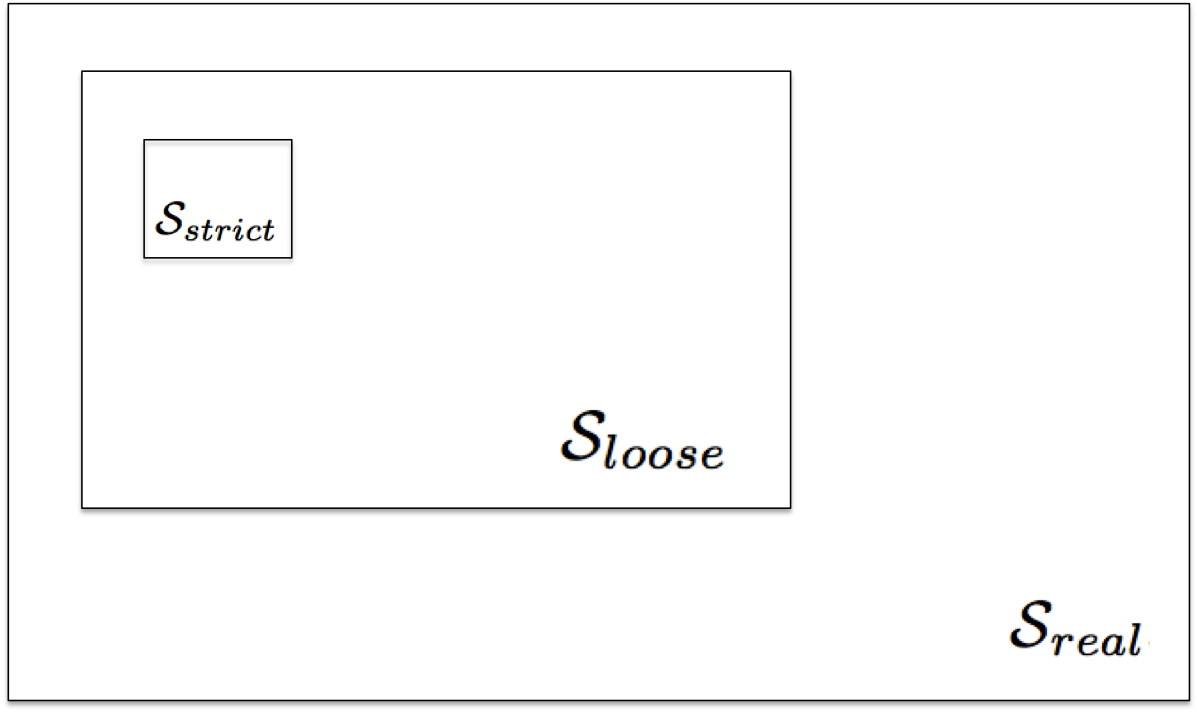
\includegraphics[width=\columnwidth]{Figures/dataset_sizes.png}
	\caption{Representation of our $\mathcal{S}_{strict}$, $\mathcal{S}_{loose}$ and $\mathcal{S}_{real}$ scenarios.}
	\label{fig:dataset_sizes}
\end{figure}

Problema de cyber ataques, frequencia, detecçao.

Problema do malware, quantidade, dificuldade em detectar

Aplicaçao de tecnicas de ML para detectar malware, com resultados bons


%%%%%%%%%%%%%%%%%%%%%%%%%%%%%%%%%%%%%%%%%%%%%%%%%%%%%%%%%%%%%%%%%%%%%%%%
\section{Motivation}
\label{section:motivation}

Como ja foi referido, problema do malware, quantidade, dificuldade distinguir.

Bastante trabalho ja feito em malware detection com base em ML, mas com pouca enfase na consistencia temporal das amostras, malware evolve ao longo do tempo.

%%%%%%%%%%%%%%%%%%%%%%%%%%%%%%%%%%%%%%%%%%%%%%%%%%%%%%%%%%%%%%%%%%%%%%%%
\section{Main Goal}
\label{section:overview}

Pelas razoes ja descritas, o objectivo desta tese é desenvolver um modelo de ML para detectar malware, mas tendo em conta a consistencia temporal.


%%%%%%%%%%%%%%%%%%%%%%%%%%%%%%%%%%%%%%%%%%%%%%%%%%%%%%%%%%%%%%%%%%%%%%%%
\section{Thesis Outline}
\label{section:outline}

Chapter \ref{chapter:related_work} introduces malware by describing some of its history, followed by different techniques to detect malware. We then describe a practical application of a specific analysis technique, from which we obtained our dataset.
We introduce the notion of machine learning and its applications, followed by related work that specifically uses \gls{ml} to detect malware. 

Chapter \ref{chapter:data_collection} describes our initial approach and methodology to help solve the problem of malware detection using \gls{ml}. We detail the data gathering process and how it was analyzed, followed by the labeling process and dataset creation.

Chapter \ref{chapter:static_features} and \ref{chapter:dynamic_features} takes the created datasets to build a malware detection model based on both static and dynamic features, as well as how these perform under different validation methodologies.

Chapter \ref{chapter:practical_applications} describes how our model is practically implemented both as an online malware detection service (identical to Malwr) and how it was inserted into a corporate email server to analyze attachments.

Chapter \ref{chapter:conclusions} provides some final remarks on our work and contributions, together with possible ideas that may improve the presented work.
